\documentclass[11pt]{beamer}
%\usefonttheme{professionalfonts}
\usefonttheme{serif}

\usepackage[utf8]{inputenc}
\usepackage[T1]{fontenc}
\usepackage{lmodern}
\usepackage[spanish]{babel}
\usepackage{amsmath}
\usepackage{amssymb}
\usetheme{EastLansing}
\usepackage{graphicx}
\usepackage[]{xcolor}
\usepackage{tikz}
%\usepackage[table]{xcolor}
\usepackage{colortbl}
\usetikzlibrary{shapes.geometric, arrows}

\author{Dr. Alejandro Rodriguez}
\title{Probabilidad y Estad\'istica\\Probabilidad}
\subtitle{Universidad Tecnol\'ogica Iz\'ucar de Matamoros\\UTIM }


\begin{document}

    \begin{frame}[plain]
        \maketitle
    \end{frame}

    \begin{frame}{Temas de Probabilidad}
      \begin{itemize}
          \item Conjuntos
          \item Probabilidad Básica y Condicional
          \item Distribuciones Discretas de Probabilidad
          \item Distribuciones Continuas de Probabilidad
          \item Distribuciones Muestrales
      \end{itemize}
    \end{frame}
    \begin{frame}{Probabilidad}
       \begin{block}{Probabilidad}
           El término \textbf{probabilidad} se refiere al estudio de azar y la incertidumbre en cualquier
           situación en la cual varios posibles sucesos pueden ocurrir.
       \end{block}
       \pause
       En palabras simples, fenómenos aleatorios son los que pueden dar lugar a varios resultados, sin que pueda ser posible enunciar con certeza cuál de éstos va a ser observado en la realización del experimento.
    \end{frame}



    \section*{Conjuntos}
      \begin{frame}{Espacio muestral}
          \begin{block}{title}
              Definir los conceptos y notación de conjuntos:
              -Universo
              -Vacío
              -Subconjunto

              Describir el proceso de construcción del diagrama de Venn Euler.

              Explicar las operaciones entre conjuntos:
              - Unión
              - Intersección
              - Complemento
              - Diferencia
          \end{block}
      \end{frame}
      \subsection*{Espacio Muestral}
        \begin{frame}{Conjuntos o espacio muestral}
          \begin{block}{Espacio muestral}
              El \textbf{espacio muestral} de un experimento denotado por $E$ , es el \textbf{conjunto} de todos los posibles resultados de dicho experimento.
          \end{block}
          \pause
          Ejemplos:
          \begin{enumerate}[<+->]
              \item El espacio muestral asociado a lanzar un dado, E = {1,2,3,4,5,6}
              \item El espacio asociado a preguntar a un cliente si le gusta o no nuestro producto es E ={S, N} (S – sí; N – no)
              \item El espacio asociado a indagar si 3 clientes que entraron a una tienda compraron un producto es E = {SSS, SSN, SNS, NSS, SNN, NSN, NNS, NNN}.
          \end{enumerate}
        \end{frame}
      \subsection*{Suceso o evento}
        \begin{frame}{Conjuntos: Suceso o evento}
          \begin{block}{Suceso o evento}
              Un \textbf{suceso} o \textbf{evento} es cualquier recopilación (\textbf{subconjunto}) de resultados contenidos en el espacio muestral $E$. Un evento es \textit{simple} si consiste en exactamente un resultado y \textit{compuesto} si consiste en más de un resultado.
          \end{block}
          \pause
          Dado que los sucesos son subconjuntos del espacio muestral, son muy útiles los diagramas de Venn para su representación:
          \begin{figure}
              \centering
              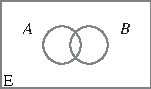
\includegraphics[width=0.3\linewidth]{images/estadistica1}
              \caption{Ejemplo de un diagrama de diagramas de Venn. E. Espacio muestral, A y B representan conjuntos o subconjuntos. }
              \label{fig:estadistica1}
          \end{figure}
        \end{frame}
      \subsection*{Propiedades de conjunto}
        \begin{frame}{}
          \begin{block}{Propiedades de conjunto}
              \begin{enumerate}[<+->]
                  \item El complemento de un evento A, denotado por A', es el conjunto de todos los resultados en \textbf{E} que no están contenidos en A.
                  \item La unión de dos eventos A y B, denotados por A $\cup$ B y leídos “A o B”, es el evento que consiste en todos los resultados que están en A o en B o en ambos eventos (de tal suerte que la unión incluya resultados donde tanto A como B ocurren, así también resultados donde ocurre exactamente uno), es decir, todos los resultados en por lo menos uno de los eventos.
                  \item La intersección de dos eventos A y B, denotada por A $\cap$ B y leída “A y B”, es el evento que consiste en todos los resultados que están tanto en A como en B.
              \end{enumerate}
          \end{block}
        \end{frame}

        \begin{frame}{Unión}
          \begin{figure}
              \centering
              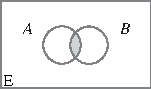
\includegraphics[width=0.7\linewidth]{images/estadistica2}
              \caption{Unión: La región sombreada es A $\cup$ B.}
              \label{fig:estadistica2}
          \end{figure}

        \end{frame}
        \begin{frame}{Intersección}
          \begin{figure}
            \centering
            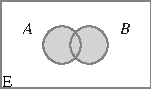
\includegraphics[width=0.7\linewidth]{images/estadistica3}
            \caption{Intersección: La región sombreada es A $\cap$ B}
            \label{fig:estadistica3}
          \end{figure}

        \end{frame}
        \begin{frame}{Complemento}
          \begin{figure}
            \centering
            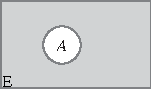
\includegraphics[width=0.7\linewidth]{images/estadistica4}
            \caption{Complemento: La región sombreada es A'. }
            \label{fig:estadistica4}
          \end{figure}

        \end{frame}
        \begin{frame}{Mutuamente excluyentes}
        \begin{figure}
            \centering
            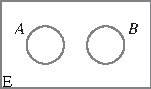
\includegraphics[width=0.7\linewidth]{images/estadistica5}
            \caption{Eventos mutuamente
excluyentes.}
            \label{fig:estadistica5}
        \end{figure}

      \end{frame}

        \begin{frame}{Mutuamente excluyentes}
           \textbf{\begin{center}
                 \huge TO BE CONTINUE
        \end{center}}
        \end{frame}


    \section*{Probabilidad Básica y Condicional}
      \subsection*{Métodos para el cálculo de probabilidad}
        \begin{frame}{Probabilidad}
            \begin{block}{Probabilidad}
                El término \textbf{probabilidad} se refiere al estudio de azar y la incertidumbre en cualquier
                situación en la cual varios posibles sucesos pueden ocurrir.
            \end{block}

            En palabras simples, fenómenos aleatorios son los que pueden dar lugar a varios resultados, sin que pueda ser posible enunciar con certeza cuál de éstos va a ser observado en la realización del experimento.
        \end{frame}

        \begin{frame}{}
            \begin{center}
                \textbf{\huge Cálculo de probabilidad}
            \end{center}
        \end{frame}

        \begin{frame}{Cálculo de probabilidad}
            La noción de probabilidad tiene cuatro acepciones básicas:
            \\
            \begin{itemize}[]
                \item Empírica (práctica, relacionada con la frecuencia relativa)
                \item Clásica (teórica, relacionada con casos equiprobables)
                \item Axiomática (basada en un modelo matemático)
                \item Intuitiva (relacionada con experiencias o mediciones subjetivas)
            \end{itemize}
        \end{frame}






        \subsubsection*{Método Empírico}
          \begin{frame}{Método empírico}
            J. J. Bernoulli, observando los resultados del lanzamiento de una moneda un número grande de veces, notó que el número de caras y cruces tendía a igualarse. Es decir, que la frecuencia relativa de la obtención de caras se acercaba más al número de cruces, cuanto mayor era el número de lanzamientos, dicho de otra manera, las frecuencias relativas se parecían cada vez más a 0.5. De aquí la definición empírica de Probabilidad:
            \begin{block}{Probabilidad}
               \textbf{Probabilidad} de un suceso es el número al que tiende la frecuencia relativa asociada al suceso a medida que el número de veces que se realiza el experimento crece.
               $$P(A) = \lim_{N \to \infty }\dfrac{n(A)}{N} $$
            \end{block}
          \end{frame}


           \begin{frame}{Método empírico}
               \begin{block}{Ejemplo}
                   En una línea de envasado de cereales se tienen los siguientes registros de envases defectuosos:
                   \begin{table}[!h]
                       \centering
                       \begin{tabular}{|c|c|c|c|c|c|}
                           \hline
                           Semana & 1 & 2 & 3 & 4 & Total\\
                           \hline
                           Envases recibidos  & 1200 & 1350 & 1150 & 1100 & 4800\\
                           Envases rechazados & 4    & 6    & 4    & 5    & 19\\
                           \hline
                       \end{tabular}
                   \end{table}
                   Determine la probabilidad de encontrar un envase defectuoso.
               \end{block}
               \pause
               \textbf{Solución:}\\
               Evidentemente la frecuencia relativa de ocurrencia de este suceso es igual a $19/4800 = 0.004$ o lo que es lo mismo de un 0.4\%.
           \end{frame}



        \subsubsection*{Método Clásico}


          \begin{frame}{Probabilidad Clásica (Definición de Laplace)}
            \begin{block}{Enfoque clasico}
               Es el \textbf{\textit{número de casos favorables al evento}} (es decir, resultados posibles del evento o prueba que hacen que ocurra el evento) \textit{\textbf{entre el número de casos posibles}} (o sea todos los resultados posibles del experimento), \textit{\textbf{pero considerando que cada uno de los casos posibles tiene igual probabilidad de ocurrir}}.
               $$P(E) = \dfrac{n(E)}{N}$$
               $n(E)$: número de casos favorables a E\\
               $N$: número de casos posibles
            \end{block}
          \end{frame}

         \begin{frame}{Probabilidad Clásica (Definición de Laplace). Ejemplo}
             Ejemplo: El evento que consiste en obtener un mismo número de ambos dados al lanzar dos dados tiene probabilidad
             $$P(E) = \dfrac{6}{36} = \dfrac{1}{6}$$
             \pause
             \begin{table}[!h]
               \centering
               \begin{tabular}{|c|c|c|c|c|c|}
                   \hline
                   \cellcolor{blue!25} 11 & 21 & 31 & 41 & 51 & 61 \\
                   \hline
                   12 & \cellcolor{blue!25} 22 & 32 & 42 & 52 & 62 \\
                   \hline
                   13 & 23 & \cellcolor{blue!25} 33 & 43 & 53 & 63 \\
                   \hline
                   14 & 24 & 34 & \cellcolor{blue!25} 44 & 54 & 64 \\
                   \hline
                   15 & 25 & 35 & 45 & \cellcolor{blue!25} 55 & 65 \\
                   \hline
                   16 & 26 & 36 & 46 & 56 & \cellcolor{blue!25} 66 \\
                   \hline
               \end{tabular}
             \end{table}
             \begin{center}
                 Combinaciones: 36
             \end{center}
         \end{frame}





        \subsubsection*{Método Subjetivo o Intuitivo}
          \begin{frame}{Método Subjetivo o Intuitivo}
            Hay otro tipo de probabilidades como la llamada probabilidad \textbf{subjetiva} o \textbf{intuitiva} que es una cierta evaluación personal de la probabilidad, en lugar de ser teórica o experimental. Por ejemplo, si se desea opinar acerca de las posibilidades de que llueva en mayo en Izúcar de Matamoros, uno puede opinar, de acuerdo a la experiencia propia, acorde con los años en que ha residido en un lugar, por ejemplo que mañana es posible que la probabilidad de lluvia sea de un 20 \%, muy distinta a la que pudiera decir la misma persona si le preguntan en junio, un mes en el que comienzan las lluvias por esta región de Izúcar. No obstante, en ciertos estudios y situaciones los criterios de los expertos pueden utilizarse y manejarse incluso utilizando métodos estadísticos.
          \end{frame}

      \subsection*{Técnicas de conteo}

        \begin{frame}{}
           \begin{center}
               \textbf{\huge Técnicas de conteo}
           \end{center}
        \end{frame}

        \begin{frame}{Técnicas de conteo}
            Para utilizar el enfoque clásico de la probabilidad (a priori), es necesario conocer el numero total de resultados de una muestra o experimento.

            Las \textbf{técnicas de conteo} generalmente se utilizan como un medio para determinar el número total de resultados y son empleadas cuando realizar el conteo de forma manual se hace complicado.
            \pause
            \begin{block}{Técnicas de conteo}
                Las \textbf{Técnicas de conteo} son una serie de métodos de probabilidad para contar el número posible de arreglos dentro de un conjunto o varios conjuntos de objetos
            \end{block}
            \begin{itemize}
                \item Diagrama de Árbol
                \item Regla multiplicativa
                \item Combinación
                \item Permutación
            \end{itemize}
        \end{frame}



        \subsubsection*{Diagrama de Árbol}
          \begin{frame}{Diagrama de Árbol}
            Un diagrama de árbol es una representación gráfica de los posibles resultados de un experimento que tiene varios pasos.
            \begin{figure}
                \centering
                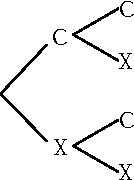
\includegraphics[width=0.3\linewidth]{images/estadistica6}
                \caption{Lanzamiento de una monada, dos veces consecutivas.}
                \label{fig:estadistica6}
            \end{figure}

          \end{frame}
          \begin{frame}{Diagrama de Árbol}
              \begin{figure}
                  \centering
                  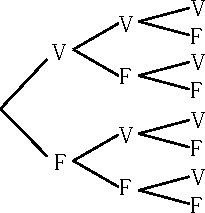
\includegraphics[width=0.3\linewidth]{images/estadistica7}
                  \caption{Posibles respuestas  de V o F, en un examen de tres preguntas.}
                  \label{fig:estadistica7}
              \end{figure}

          \end{frame}
        \subsubsection*{Regla multiplicativa}
          \begin{frame}{Regla multiplicativa}
            \begin{block}{Regla multiplicativa}
                Si una operación puede realizarse en $n_i$ formas, y si por cada una de éstas una segunda operación puede llevarse a cabo en $n_2$ formas, entonces las dos operaciones pueden realizarse juntas en $n_1n_2$ formas.
            \end{block}
            \begin{block}{Ejemplo}
                ¿Cuantos puntos muetrales hay en una espacio muestral cuando se lanza un par de dados una sola vez?
                \pause
                \textbf{Solución}: El primer dado puede caer en cualquiera de $n_1 = 6$ formas. Para cada una de éstas el segundo puede, también, caer en $n_2 = 6$ formas. Por tanto el par de dados pueden caer:
                $$ n_1n_2 = (6)(6) = 36 $$
            \end{block}
          \end{frame}
        \subsubsection*{Combinación}
          \begin{frame}{Combinación}
            content...
          \end{frame}
        \subsubsection*{Permutación}
          \begin{frame}{Permutación}
            content...
          \end{frame}


      \subsection*{Conceptos de probabilidad}

    \section*{Distribuciones Discretas de Probabilidad}
    \begin{frame}{title}
        content...
    \end{frame}



    \section*{Distribuciones Continuas de Probabilidad}
    \begin{frame}{title}
        \begin{block}{title}
            content...
        \end{block}
    \end{frame}



    \section*{Distribuciones Muestrales}
    \begin{frame}{title}
        \begin{block}{title}
            content...
        \end{block}
    \end{frame}


\end{document}